\documentclass{beamer}

\usepackage[utf8]{inputenc}
\usepackage[T1]{fontenc}
\usepackage{graphicx}
\usepackage{multimedia}
\usepackage{booktabs}

\usetheme{uoit}

\title[Amazing Thesis Work]{Really, Really Amazing Thesis Work}

\author{Marvin Martian}
\institute[uoit]
{
  Mechatronics and Robotics Laboratory \\
  University of Ontario Institute of Technology \\
  \medskip
  \textit{marvin.martian@uoit.ca}
}
\date{\today}

\begin{document}

  \begin{frame}
    \titlepage
  \end{frame}

  \begin{frame}{Overview}
    \tableofcontents
  \end{frame}

  \section{First section}

    \subsection{First sub-section}
    
      \begin{frame}{List}
        \begin{itemize}
        \item Try to use
        \item points in a list
        \item to convey your
        \item points.
        \end{itemize}
      \end{frame}

      \begin{frame}{Blocks}
        \begin{block}{Block 1}
          Make a BOLD statement using blocks.
        \end{block}
        \begin{block}{Block 2}
          BLOCK 2
        \end{block}
      \end{frame}

      \begin{frame}{Multiples Columns}
        \begin{columns}[c]
          \column{.45\textwidth} % Left column and width
          \textbf{Ordered list}
          \begin{enumerate}
            \item One
            \item Two
            \item Three
          \end{enumerate}
          \column{.5\textwidth} % Right column and width
          Plain text.
        \end{columns}
      \end{frame}

  \section{Second section}

    \begin{frame}{Table}
      \begin{table}[h]
      \centering
      \caption{Modified Denavit-Hartenberg Parameters}
        \begin{tabular}{cccccc}
          \toprule
          $F_{i-1}$ & $a_{i-1}$ & $\alpha_{i-1}$ & $d_i$ & $\theta_i$ & $F_i$ \\
          \midrule
          0 & 0 & 0 & $l_1$ & $\theta_1$ & 1 \\
          1 & 0 & $\pi/2$ & 0 & $\theta_2$ & 2 \\
          2 & $l_2$ & 0 & 0 & $\theta_3$ & 3 \\
          3 & $l_3$ & 0 & 0 & $\theta_4$ & 4 \\
          4 & $l_4$ & 0 & 0 & 0 & G \\
          \bottomrule
        \end{tabular}
      \label{tab:dh}
      \end{table}
    \end{frame}

    \begin{frame}{Equations}
      \begin{equation}
        \label{eq:1}
        r_{c1} = \frac{2r^2(1-\cos\theta_x)-h^2_{xx}}{2r(\cos\theta_x-1)}
      \end{equation}
    \end{frame}

    \begin{frame}{Figure}
      \begin{figure}
        
\includegraphics[scale=1.0]{uoit.png}
        \caption{UOIT logo}
      \end{figure}
    \end{frame}

    \begin{frame}{Video}
      \begin{figure}[h!]
        \centering
        \movie[label=show3,width=1.0\textwidth,poster
               ,autostart,showcontrols,loop]
          {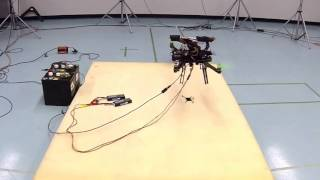
\includegraphics[width=1.0\textwidth]{ams.jpg}}{ams.mp4}
          \caption{AMS Test}
      \end{figure}
    \end{frame}

  \section{Third Section}

    \begin{frame}{Citation}
      Cite who's work helped you \cite{oldThesis}.
    \end{frame}

    \begin{frame}[allowframebreaks]{References}
      \bibliographystyle{IEEEtran}
      \bibliography{references.bib}
    \end{frame}

    \begin{frame}
      \Huge{\centerline{The End}}
    \end{frame}

\end{document}
